% % no answer key
% \documentclass[letterpaper]{exam}

% answer key
\documentclass[letterpaper, landscape]{exam}
\usepackage{2in1, lscape} 
\printanswers

\usepackage{units} 
\usepackage{xfrac} 
\usepackage[fleqn]{amsmath}
\usepackage{cancel}
\usepackage{float}
\usepackage{mdwlist}
\usepackage{booktabs}
\usepackage{cancel}
\usepackage{polynom}
\usepackage{caption}
\usepackage{fullpage}
\usepackage{comment}
\usepackage{enumerate}
\usepackage{graphicx}
\usepackage{parskip}

\everymath{\displaystyle}


\title{Statistics \\ Homework Six}
\date{\today}
\author{}

\begin{document}

  \maketitle

  \section{Homework}
    \begin{itemize*}
      \item read Chapter 6 
      \item take a look at the ``Check Your Skills'' exercises
      \item exercises: 19-24, 27, 29-31
    \end{itemize*}

  \ifprintanswers
    \begin{description}

      \item[19]     
        \begin{figure}[H]
          \centering
          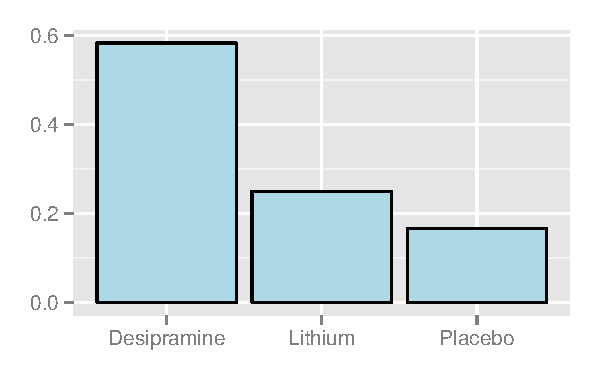
\includegraphics[scale = 0.8]{figures/ex19.pdf}
          \caption{Exercise 19}
          \label{fig:ex19}
        \end{figure}

        \begin{table}[H]
          \centering
          \begin{tabular}{rlr}
            \toprule
              & Treatment   & Success \\
            \midrule
            1 & lithium     & 25\% \\
            2 & placebo     & 17\% \\
            3 & desipramine & 58\% \\
            \bottomrule
          \end{tabular}
          \caption{Exercise 19}
          \label{tab:ex19}
        \end{table}

        \begin{parts}
          \part Figure \ref{fig:ex19}
          \part Table \ref{tab:ex19}
        \end{parts}

      \item[20]
        \begin{table}[H]
          \centering
          \begin{tabular}{lr}
            \toprule
            Job Grade & Percent \\
            \midrule
            1         & 12\% \\
            2         & 51\% \\
            3         & 30\% \\
            4         & 7\% \\
            \bottomrule
          \end{tabular}
          \caption{By Job Grade}
        \end{table}

        \begin{table}[H]
          \centering
          \begin{tabular}{lr}
            \toprule
            Marital Status & Percent \\
            \midrule
            single         & 4\% \\
            married        & 94\% \\
            divorced       & 2\% \\
            widowed        & 1\% \\
            \bottomrule
          \end{tabular}
          \caption{By Marital Status}
        \end{table}

      The percentages might not add up to exactly 100\% because of rounding, but
      they should be close.
      
    \item[21]
      There are 58 single men with grade 1 jobs and 955 grade 1 jobs, 
      \[
        58/955 \approx 6 \%
      \]
      of the grade 1 jobs are held by single men.

      There are 58 single men with grade 1 jobs and 337 single men, 
      \[
        58/337 \approx 17 \% 
      \]
      of the single men hold grade 1 jobs.

    \item[22]
      \begin{table}[H]
        \centering
        \begin{tabular}{rr}
          \toprule
          job grade & percentage \\
          \midrule
          1         & 17.2  \\
          2         & 65.9  \\
          3         & 14.8  \\
          3         & 2.1   \\
          \bottomrule
        \end{tabular}
      \end{table}

      The percentages should (and do) add up to 100\%.

    \item[23]
      \begin{parts}
        \part There are 7730 married men and only 337 single men, so you would expect
        more married men than single men in all the job categories.

        \part 

          \begin{table}[H]
            \centering
            \begin{tabular}{rlrrrrr}
              \toprule
                & marital status & 1    & 2    & 3    & 4    \\
              \midrule
              1 & single         & 17.2 & 65.9 & 14.8 & 2.1 \\
              2 & married        & 11.3 & 50.8 & 31.0 & 6.9 \\
              3 & divorced       & 11.9 & 55.6 & 27.0 & 5.6 \\
              4 & widowed        & 19.0 & 47.6 & 23.8 & 9.5 \\
              \bottomrule
            \end{tabular}
          \end{table}

          There are more single men than married or divorced in grade 1 job.  
          Single men tend to be younger, so this just means the single men tend to
          have the entry-level jobs.  There are few single men with grade 4 jobs,
          which makes sense for the same reason.

          The widowed category doesn't fit the pattern, but there are very few
          widowed men, so there probably isn't a large enough sample size to get a
          good picture of the widowed men.

      \end{parts}

    \item[24] As you get older, you tend to make more money.  As you get older, you
      are also more likely to get married.  Age is probably the lurking variable.

    \item[27]
      \begin{table}[H]
        \centering
        \begin{tabular}{rlrrr}
          \toprule
            & Degree & 1    & 2    & 3     \\
          \midrule
          1 & BA     & 45.0 & 47.2 & 7.8  \\
          2 & HS     & 29.7 & 49.6 & 20.7 \\
          3 & No HS  & 24.4 & 38.6 & 37.0 \\
          \bottomrule
        \end{tabular}
      \end{table}

      The more education you have, the more freedom you have in organizing your work.

    \item[30]
      \begin{table}[H]
        \centering
        \begin{tabular}{rlrrr}
          \toprule
            & Oil  & colon & control & rectal \\
          \midrule
          1 & high & 20.7  & 67.9    & 11.4 \\
          2 & low  & 19.7  & 67.9    & 12.4 \\
          3 & med  & 19.7  & 68.3    & 12.0 \\
          \bottomrule
        \end{tabular}
      \end{table}

      It doesn't look like oil consumption has much affect on cancer rates.

    \item[31]
      \begin{table}[H]
        \centering
        \begin{tabular}{rlrr}
          \toprule
            & Anger & No CHD & CHD \\
          \midrule
          1 & high  & 95.7   & 4.3 \\
          3 & mod   & 97.7   & 2.3 \\
          2 & low   & 98.3   & 1.7 \\
          \bottomrule
        \end{tabular}
      \end{table}

      It looks like the angry people are much more likely to get heart disease than
      either of the other two categories.  The moderate anger people are also a bit
      more likely to get heart disease than the low anger people.

  \end{description}

  \else
    \vspace{10 cm}
    \begin{quote}
      \begin{em}
        I would encourage people to look around them in their community and find an
        organization that is doing something that they believe in, even if that
        organization has only five people, or ten people, or twenty people, or a hundred
        people. And to look at history and understand that when change takes place it
        takes place as a result of large, large numbers of people doing little things
        unbeknownst to one another
      \end{em}
    \end{quote}
    \hspace{1 cm} --Howard Zinn
  \fi

\end{document}

